\chapter{Algorithm}
\label{chap:11}

\section{Linear Method}
\subsection{Control System}
The control system is constructed as shown here. The main part is a closed loop control. The PID controller computes the PWM value based on the difference of reference and delivered pressure, and the valve releases with given restriction. Feed Forward offers the predicted pwm values which is obtained by experiments before so that the system could settle faster.

\begin{figure}[h]
    \centering 
    \captionsetup{justification=centering}
    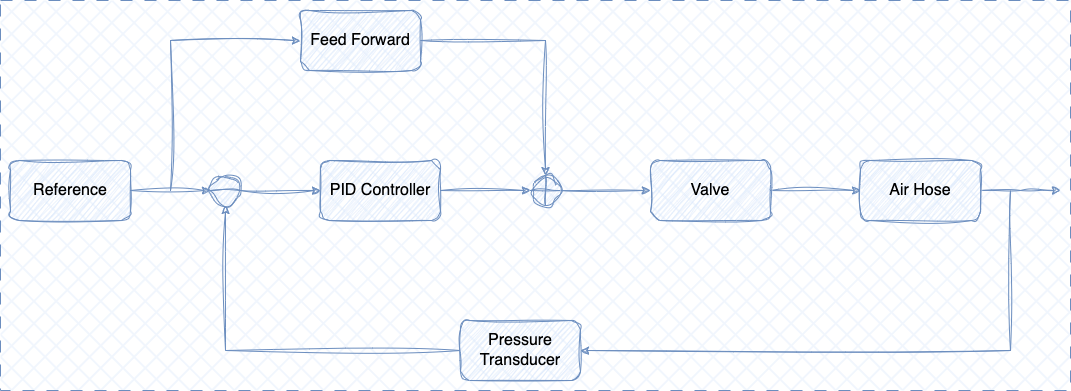
\includegraphics[width=0.75\textwidth]{img/cs_lin.png}
    \caption{a nice plot}
    \label{fig:mesh1}
\end{figure}



\subsection{State Machine}
The state machine below shows how the control system works. First the the cuff would be inflated to the target pressure. And the control magnitude of the delation would be calculated, the air would be released based on the computed restriction, and the whole process stops when the pressure is smaller than the final release pressure.

\begin{figure}[h]
    \centering 
    \captionsetup{justification=centering}
    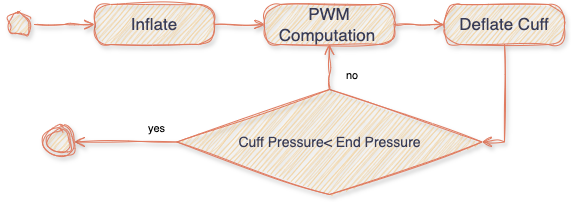
\includegraphics[width=0.75\textwidth]{img/st_lin.png}
    \caption{a nice plot}
    \label{fig:mesh1}
\end{figure}

\subsection{PID Control}

 PID control is a control mechanism widely used industrial control systems and applications requiring continuously modulated control. It is short of proportional integral and derivation. P factor provides the response to error, increasing P the system can react faster, but using p factor alone would also generate a large overshoot while reducing the rise time. But in steady state, the error is also steady so P factor alone cannot eliminate the steady error. I factor can eliminate the steady error by adding the control effect, when the error is eliminated, the integral term will cease to grow. And D factor can reduce the oscillation and overshoot by  reducing the effect of the error. 

 To get the error, the set point must be taken care first, the slope would be calculated base on the time and final pressure, and the reference pressure would be derived. The error is the difference between current pressure and the calculated reference pressure. And the most time consuming part is to figure out the proper factors. First I set all factors to 0 and then starts with P, first I increase it to 100 and then 1000 if the effect when the change is not much or getting worse I will stop and starts the tuning of I.

 \subsubsection{Digital PID}
 
\subsection{Feed Forward}

But in our case, the error at the beginning is 0 if you can still recall the equation of PID algorithm, this would leads to a zero u, which means the valve would fully open. This error is unrecoverable. FF is introduced to mitigate the problem

Instead of adjusting based not the feedback. It is based on knowledge about the process in the form of a mathematical model of the process and knowledge. Let's take the shower as an example. To have a pleasant shower, the temperature of the water is important. But we take shower in a new place, we would spend more time in adjusting the temperature of the water by switching the knob. But if we do not have to it next time since the the knob is pre-defined and if the temperature is not warm enough, we could adjust from the pre-defined place which would take much less time. In our case, the pwm values vary in a certain range when the volume deflates linearly, so we applied linear regression to fit the curve and send it to the system as the feed forward signal.  

\subsection{Filter}
 As it shown in Figure 4, when the pressure is steady, raw data from the sensor oscillate a lot, this would lead more oscillation in the control algorithm. As it indicates in the orange curve, the filter could smooth the data and not suppress the change on the pressure.

 \begin{figure}[h]
    \centering 
    \captionsetup{justification=centering}
    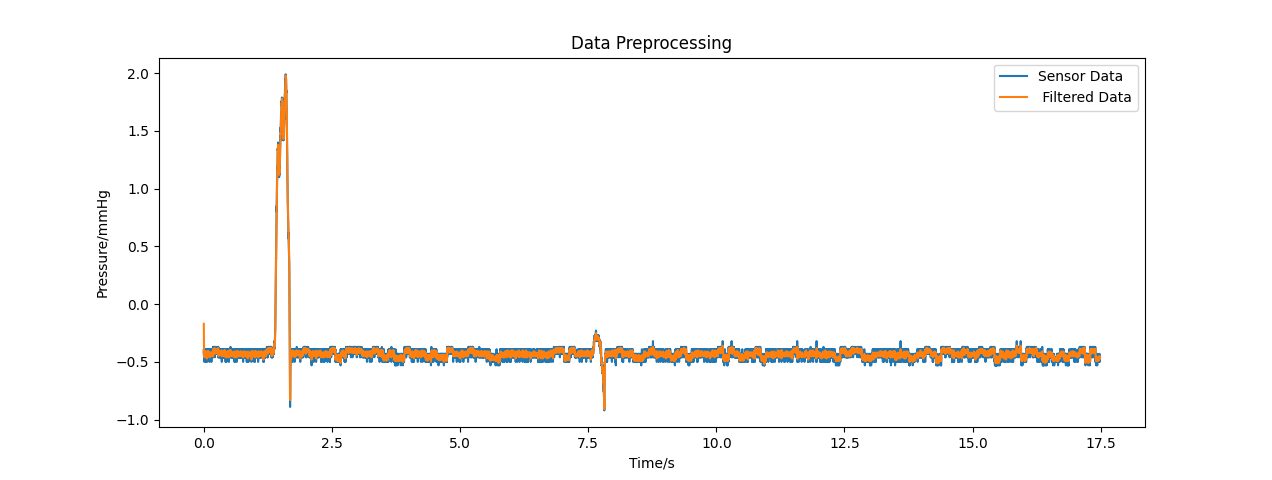
\includegraphics[width=\textwidth]{img/datapreprocessing.png}
    \caption{a nice plot}
    \label{fig:mesh1}
\end{figure}


\section{Differential Method}
\subsection{Control System}
Here is the control system, two linearization control systems are combined together. One would deflate linearly like before and the baseline would only deflate linearly without any disturbance, and the pressure difference between these two volumes would sampled by the differential sensor in the middle which has a smaller range.

\begin{figure}[h]
    \centering 
    \captionsetup{justification=centering}
    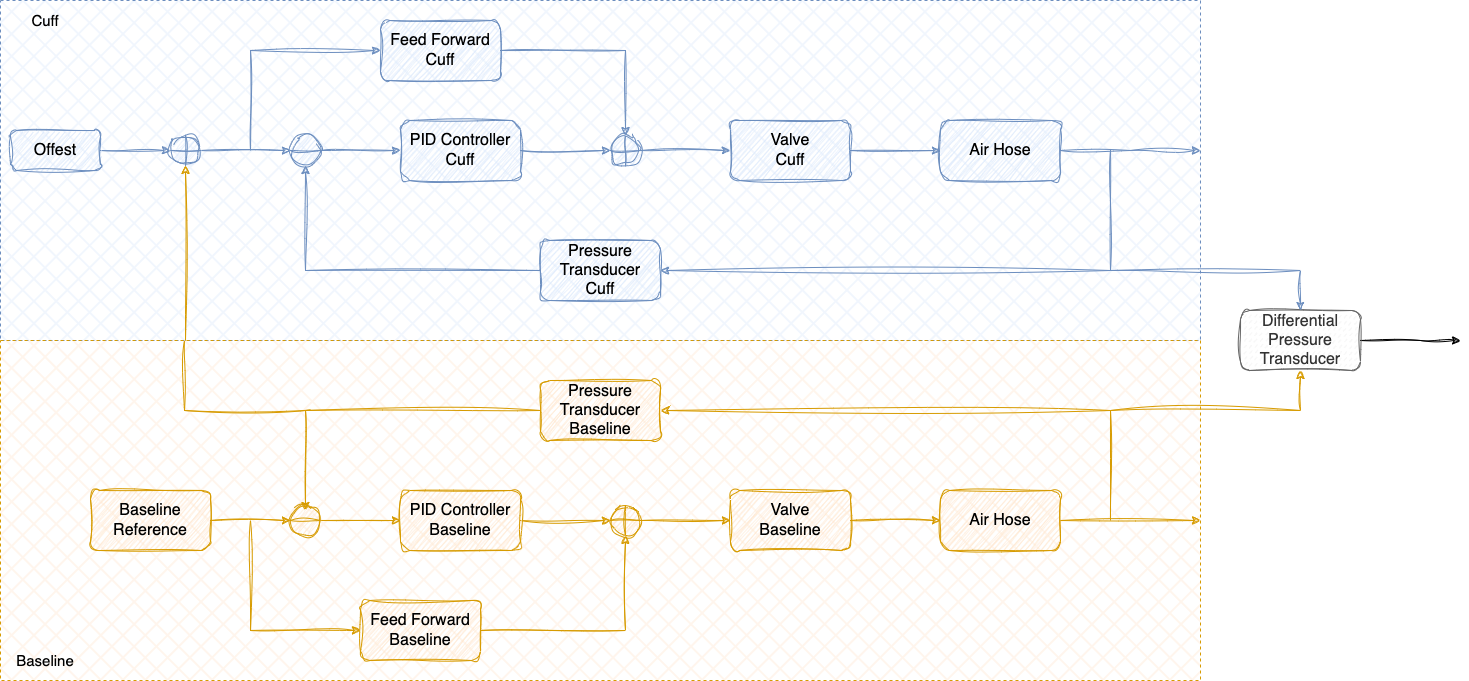
\includegraphics[width=\textwidth]{img/cs_diff.png}
    \caption{a nice plot}
    \label{fig:mesh1}
\end{figure}

\subsection{State Machine}
The state machine here shows how the control system works. First both volume would be inflated, and the middle valve would be closed to separate two volumes first during the inflation so that they have a difference in pressure. Then the linear deflation of the cuff and baseline volume would follow up. And the difference of these two volumes would be collected. Once the cuff pressure reaches the release pressure, the process stops. 

\begin{figure}[h]
    \centering 
    \captionsetup{justification=centering}
    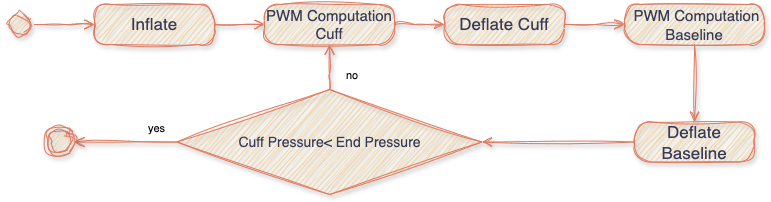
\includegraphics[width=0.75\textwidth]{img/st_diff.png}
    \caption{a nice plot}
    \label{fig:mesh1}
\end{figure}


\subsection{PID Control}
\subsection{Feed Forward}
\subsection{Filter}